\chapter{Gamma-ray Astronomy }
\label{chap:gamAstr}

\begin{figure}[h!]%[t] 
	\centering
	\makebox[\linewidth]{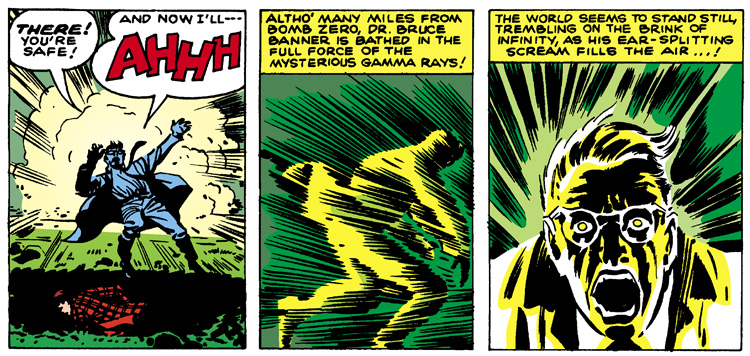
\includegraphics[width=1.\columnwidth]{Figures/panel_hulk001b}}
\end{figure}

%\begin{quote}
%	``Once there was a boy, and the boy loved stars very much'' 
%	\begin{center}---by Oliver Jeffers, from \it{How to Catch a Star} \end{center}
%\end{quote}


%ugh commentes
%\section{Introduction}\label{gamAstr:intro}


\section{\gam{} Emission Mechanisms }\label{gamAstr:Emiss}
The story of \gam{}s from astrophysical objects is a tale of the most extreme, energetic, and violent environments in our universe. \gam{}s are the highest named energy of light, starting from around several hundred\kev{} and extending up, with the highest energy \gam{}s detected being hundreds of\tev{}. Aside from the  nuclear fission, \gam{}s are produced solely by charged particles being accelerated to\gev{} and\tev{} energies and interacting with a target particle, be it other matter or photon fields.  Below we summarize the various non-thermal emission mechanisms giving rise to \gam{}s, namely, \ic{} radiation, non-thermal \brems{} (both of an accelerated electron, or leptonic, origin), and neutral pion decay emission (of an accelerated proton, or hadronic origin). We also described the \sync{} radiation process. While not typically observed up to \gam{} energies (with \sync{}  emission from the Crab nebula being an exception \cite{AbdoCrab}, with the tail of the emission extending to hundreds of\mev{}), \sync{} photons plays a significant role in understanding \ic{} \gam{} emission since the processes both arise from a shared, underlying electron population. Furthermore, observations of \sync{} emission at radio and X-ray energies is vital in  constraining a source's underlying charged particle population and the resultant \gam{} source spectra. We follow \cite{Houck06} for many of the photon emissivities given below.

\subsection{Synchrotron Radiation}\label{gamAstr:sync}
When a relativistic electron moves in a magnetic field, it experiences a force perpendicular to its velocity which causes the electron to accelerate and travel in a helical path around the magnetic field lines. This acceleration results in radiation of photons, referred to as \sync{} radiation \cite{Blumenthal70,Pacholczyk70,Rybicki86,Longair11}. The total power emitted at a frequency $\nu$ from a relativistic electron (Lorentz factor, $\gamma \gg 1$) spiraling in a magnetic field, B is:

\begin{equation}\label{eq:syncPow}
{\rm P_{emitted}(\nu) = 
\frac{\sqrt{3} q^3 B \sin\alpha}{m_e c^2} F(\nu/\nu_c) }
\end{equation}
where q is the electron's charge,  ${\rm m_e}$ is the electron's rest mass, c is the speed of light,  ${\rm \alpha }$ is the angle between the magnetic field vector and the electron's velocity vector (the pitch angle), F is called the first synchrotron function and is an integral over an irregular modified Bessel function (see \cite{Rybicki86}), and ${\rm \nu_c}$ is the frequency at which most of the power is radiated. This so-called critical frequency is:

\begin{equation}\label{eq:nuCrit}
\nu_c = \frac{3q B \gamma^2}{4\pi m_e c} 
\sin\alpha \equiv \nu_0 \gamma^2 \sin\alpha
\end{equation}
We note that the power emitted is inversely proportional to the mass, which explains the insignificance of proton synchrotron radiation, because the rest mass of the proton is $\sim$ 2000 times greater than that of the electron.

For an isotropic distribution of electrons we define  ${\rm N(p,\alpha)}$ as the number of electrons per unit solid angle and momentum with momentum p and pitch angle $\alpha$. \cite{Houck06} show that the differential photon-emissivity spectrum (\ie{}\ number of radiated photons per unit time per unit energy) is:

\begin{equation}
\frac{d n}{d \omega d t} =
\frac{\sqrt{3}q^3 B}{h m_e c^2 \nu}
\int
N(p)
R \left(\frac{\omega}{\omega_0 \gamma^2}\right)dp
\end{equation}
with $\omega$ being the radiated photon energy, ${\rm N(p) = 4\pi N(p,\alpha)}$ for an isotropic pitch-angle distribution, and
\begin{equation}
R(x) \equiv \frac{1}{2} \int_0^\pi
\sin^2 \alpha
F\left(\frac{x}{\sin\alpha}\right) d \alpha 
\end{equation}


\subsection{Non-Thermal \brems{}}\label{gamAstr:bremss}
Bremsstrahlung radiation occurs when charged particles (electron-electron or electron-ion in this case) pass near each other, causing the  primary charge to decelerate, and emit a photon. As noted by \cite{Haug75}, the electron-electron \brems{} system has no electric dipole moment, and it is the quardrapole moment that dominates in the non-relativistic regime, and thus for low energies, the electron-electron contribution is negligible. This situation changes for relativistic energies where the cross section of electron-electron \brems{} is comparable to the electron-ion cross section (where the ratio is $\simeq 0.86$ for photon energies above 10\mev{} \citep{Baring99}), thus for \gam{} studies, we include the non-thermal electron-electron component in the total \brems{} emission.

For a differential spectrum, ${\rm N_e(p)}$, corresponding to the accelerated electrons, the total emissivity is  the sum of the electron-electron and electron-ion \brems{}. The combined differential photon-emissivity spectrum is: s

\begin{equation}
{\rm \frac{d n}{d \omega d t} =
	n_e \int
	N_e(p) v_e
	\frac{d \sigma_{e e}}{d \omega}dp +
	n_Z \int
	N_e(p) v_e
	\frac{d \sigma_{e Z}}{d \omega}dp}
\end{equation}
where ${\rm d \sigma_{e Z}/d \omega}$ and ${\rm d \sigma_{e e}/d \omega}$ are the differential interaction cross sections for each interaction \citep{Koch59,Haug75}, ${\rm n_e}$ and ${\rm n_Z}$ are the stationary electron and ion densities, and ${\rm v_e}$ is the electron velocity.

\subsection{Inverse Compton Scattering}\label{gamAstr:IC}

\ic{} scattering refers to the process by which a high-energy electron collides with a lower-energy photon transferring energy and ``upscattering" the photon to higher energies \citep{Blumenthal70}. 
There are several \isrfs{} available for upscattering by a population of electrons, such as that of the \cmb{}, with a temperature ${\rm T \approx 2.73~K}$,  \fir{} dust emission (${\rm T \approx 30~K}$), and \nir{} stellar-light (${\rm T \approx 3000~K}$). While the \cmb{} component is typically dominant  in the environs of an \snr{}, \cite{Porter06} showed that the other \isrfs{} can play a significant role, for example, in the inner Galaxy or when a star forming region is nearby. For a thermal photon-field of number density $n(\omega_i)$, with $\omega_i$ being the incident and photon energy.

\begin{equation}
n(\omega_i) = 
\frac{1}{\pi^2\lambda^3} 
\frac{\omega_i^2}{e^{\omega_i/\Theta} -1}
\end{equation}
where  $\Theta=kT/(m_e c^2)$, and the Compton wavelength of the electron is $\lambda=\hbar/(m_e c)$.
For a momentum distribution of relativistic electrons, ${\rm N_e(p)}$, embedded in an isotropic photon-field of number density $n(\omega_i)$, the single-photon differential photon-emissivity spectrum is:

\begin{equation}
{\rm \frac{dn}{d\omega dt} = 
c \int  n(\omega_i)d \omega_i
\int_{p_{min}}^\infty 
N_e(p)  \sigma_{KN}(\gamma,\omega_i,\omega)dp}
\end{equation}
with $\omega$ as the upscattered photon energy, ($\omega\equiv h\nu/(m_e c^2)$), and $\sigma_{KN}$ is the Klein-Nishina scattering  cross section:
\begin{equation}
{\rm \sigma_{KN}(\gamma,\omega_i,\omega) = \frac{2\pi r_0^2}{\omega_i \gamma^2}
\left[
1 + q - 2q^2 + 2q\ln q + \frac{\Gamma^2 q^2 (1-q)}{2(1+\Gamma q)}
\right]}
\end{equation}
and,
\begin{equation}
{\rm q \equiv \frac{\omega}{4 \omega_i \gamma (\gamma-\omega)}}
\end{equation}
for ${\rm \Gamma \equiv 4\omega_i \gamma}$, and the classical electron radius, ${\rm r_0 = e^2/(m_e c^2)}$.

%\jamie{We note that in the Thomson limit, ${\rm \omega_i \ll omega \ll \gamma mc^2}$ the Klein-Nishina cross section reduces to the Thomson cross section. }


\subsection{Neutral Pion Decay Emission}\label{gamAstr:PP}
When sufficiently high-energy protons ($\approx 280\mev{}$ \cite{Dermer13}) and ions collide with interstellar material, both charged and neutral pions are created (in about equal proportions) in the aftermath. The neutral pion subsequently (and expediently; within $~10^{-16}$ s) decays into two \gam{} photons (with a branching fraction of 98.8\% \cite{Beringer12}), each of rest energy $\omega_0 =(m_{\pi}c^2)/2\approx 67.5\mev{}$. For a differential proton distribution ${\rm N_p(p)}$, the differential photon distribution is:

\begin{equation}
\frac{d n}{d \omega d t} = 
n_p \int v_p N_p(p) 
\frac{d \sigma(p_\pi, p)}{d p}dp
\end{equation}
where ${\rm n_p}$ is the density of the target protons, ${\rm d \sigma(p_\pi, p)/dp}$ the differential cross section for neutral pion production for proton collisions, and ${\rm v_p}$ the non-thermal proton velocity \citep{Hillier84,Dermer86,Aharonian00}. The peak of the distribution occurs at $\approx 67.5\mev{}$ (which is half the rest mass of the neutral pion), however the peak is broadened due to Doppler shifting of the momentum distribution of the high-energy protons. This feature shows a bilateral symmetry about the peak energy in a photon spectrum representation, but in a ${\rm \nu F_\nu}$ representation, it appears as a hardening of the spectrum at a few hundred\mev{} \citep{Stecker71,Dermer13}. This characteristic pion-decay feature is colloquially referred to as the ``pion-bump", and is a vital instrument in distinguishing the proton-emitting population from the often-overlapping \ic{} and \brems{} spectrum produced at \gam{} energies. 

\section{\gam{} Emitters}\label{gamAstr:Sources}
Despite the need for extreme environmental conditions to accelerate particles to a high-enough energy to produce \gam{}s, there are a multitude of \gam{} emitters of both Galactic and extragalactic origins. Following, we summarize a subset of these \gam{} objects, with a focus on Galactic \gam{} sources observed with the \Fermi{}-\lat{}  (see Chapter \ref{chap:FGST}, for more on the \Fermi{}-\lat{}). Figure \ref{fig:7yearSkyMap} is an all-sky map using 7 years of  \Fermi{}-\lat{} data, integrated in energy above 1\gev{}. 

\begin{figure*}[!ht]
	%\begin{centering}
	\hspace{-2.7cm}
	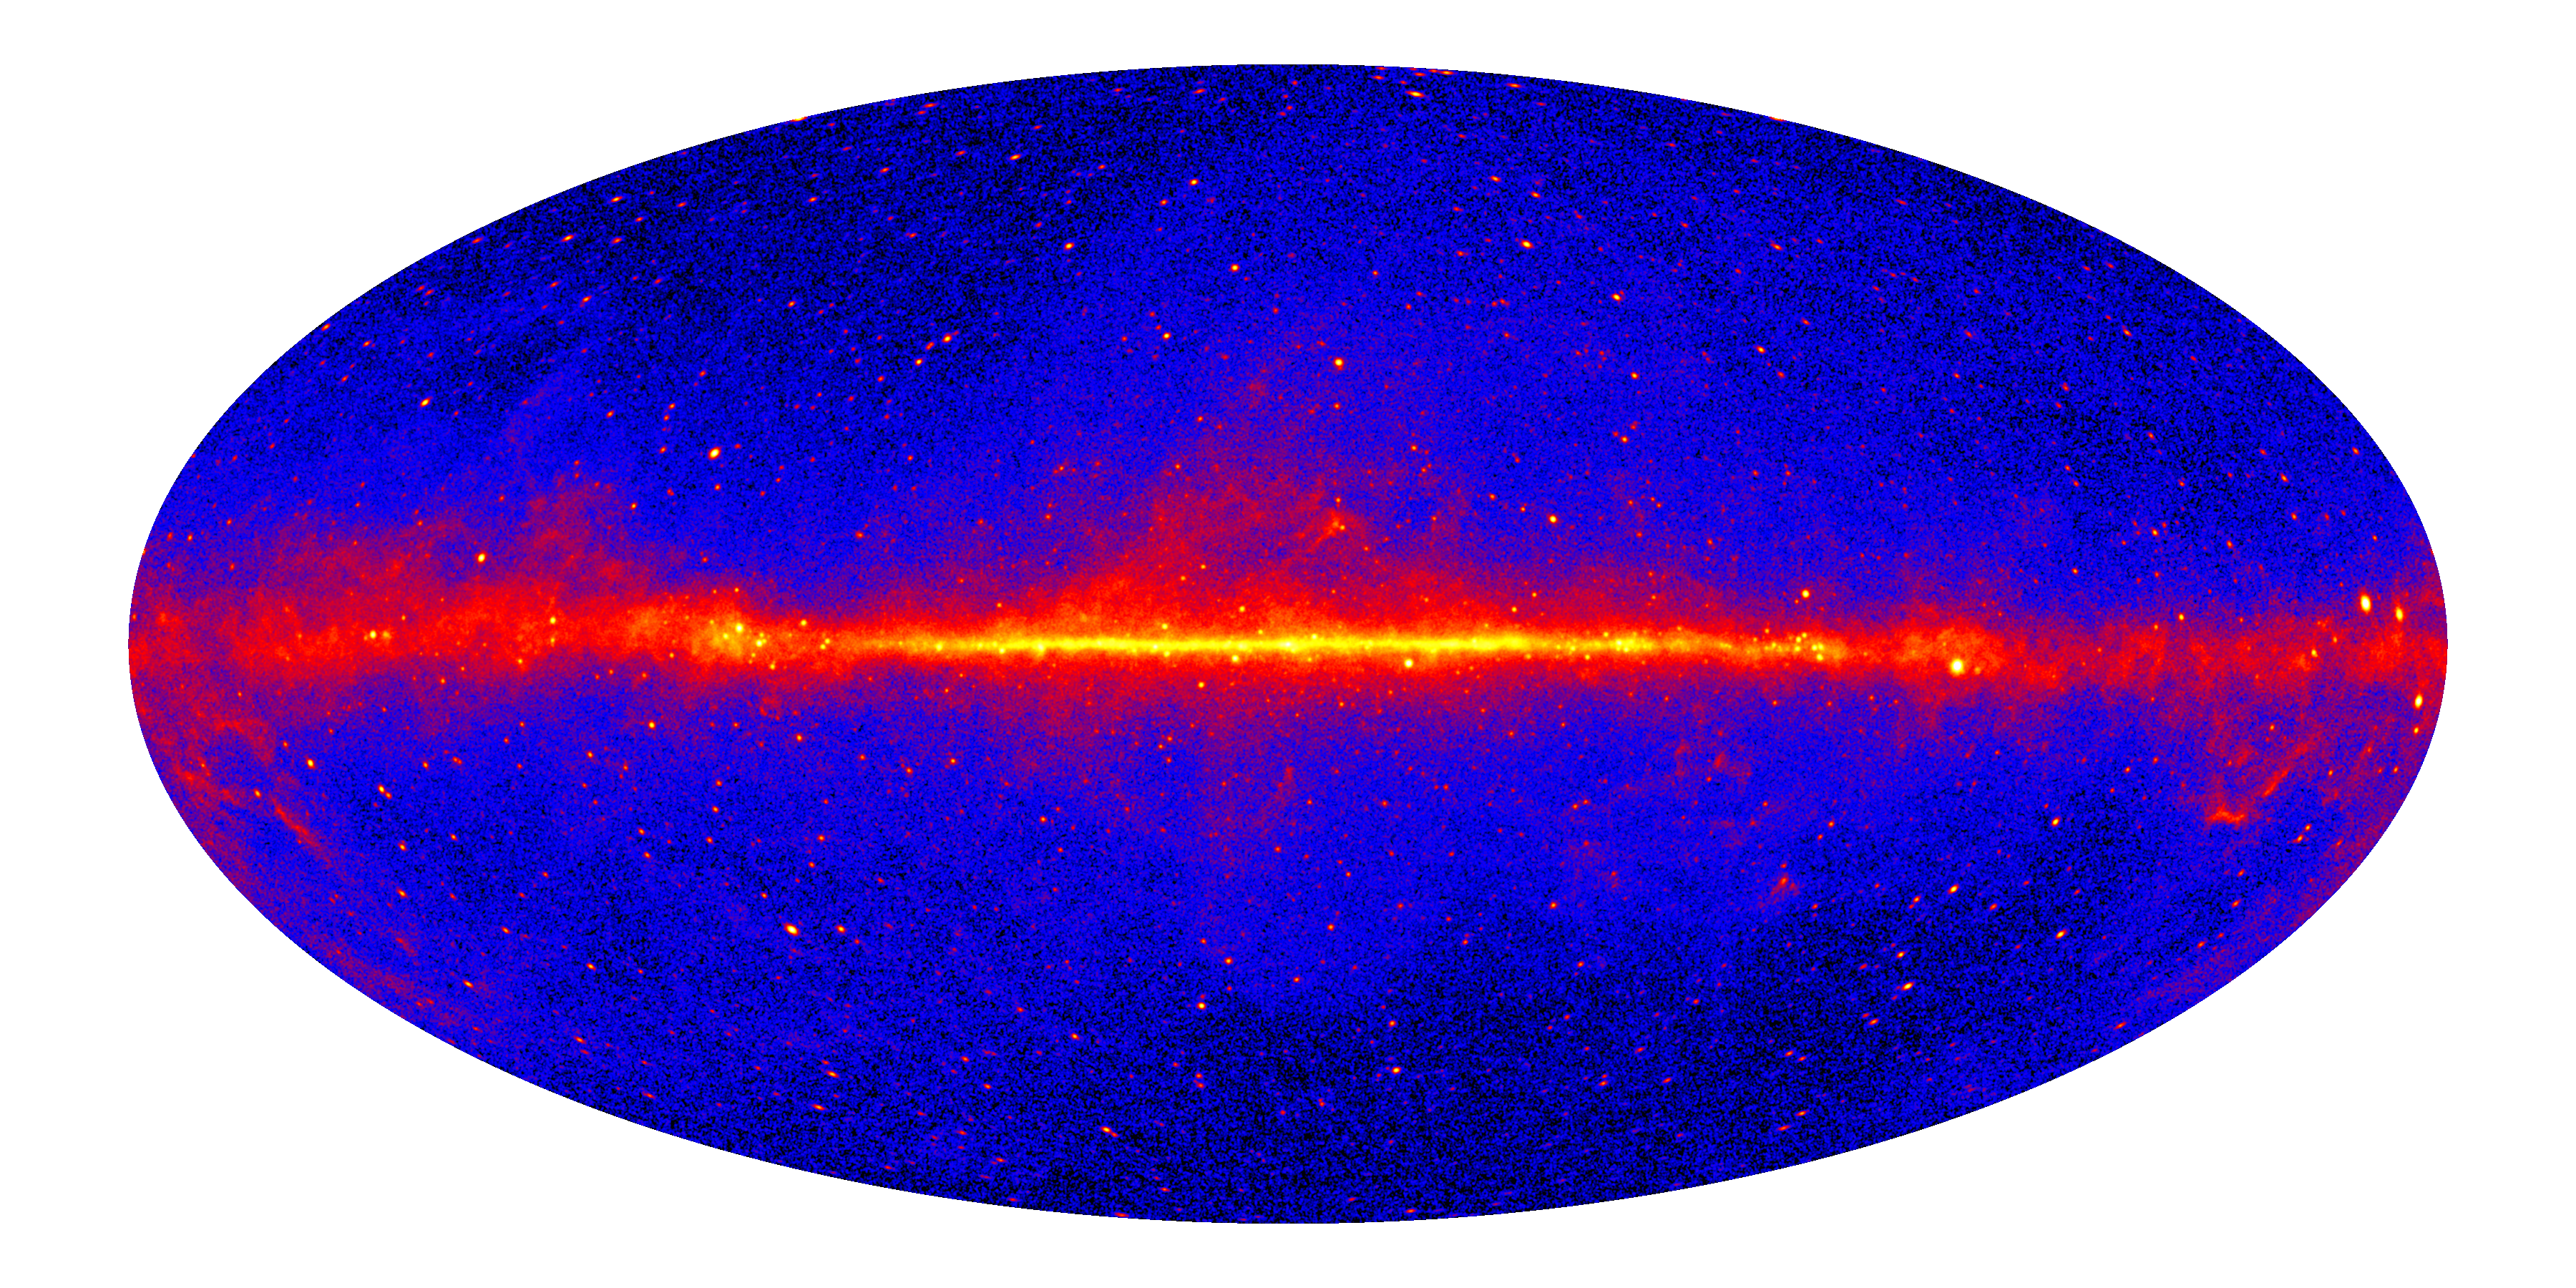
\includegraphics[width=1.3\columnwidth]{Figures/intens_ait_84m_gt1000_psf3_gal_0p1_transparent.png}
	\caption[LAT 7 year, all-sky intensity map]{\lat{}, 7 year all-sky, energy-integrated intensity map. The map is in Hammer-Aitoff projection, was created using Pass 8 Source class (PSF3 event type) photons, and the energy range of integration is $> 1\gev{}$. A logarithmic intensity scale is displayed with minimum intensity ${\rm 3.3 \times  10^{-6} ~cm^{-2}~ s^{-1}~sr^{-1}}$ and maximum intensity ${\rm 0.036 ~cm^{-2}~s^{-1}~sr^{-1}}$, for a pixel size of ${\rm 0.1^\circ / pixels}$. Image courtesy of Seth Digel and the LAT collaboration.
		\label{fig:7yearSkyMap}}
	%\end{centering}
\end{figure*}

The most prominent feature of the map shown in Figure \ref{fig:7yearSkyMap} is the central band of highly structured \gam{}s (particularly at low Galactic latitudes) corresponding to emission from the Milky Way. This radiation results from ambient \crs{} interacting with interstellar gas in the Galaxy through \brems{} and neutral pion decay processes, as well as \ic{} scattering of background radiation fields. The diffuse Galactic radiation is the dominant source of background/foreground confusion for \gam{} analysis in the Galaxy, so to properly characterize both point and spatially-extended \gam{} sources, a  model of the Galactic diffuse radiation is required. A second diffuse \gam{} background component is also apparent in Figure \ref{fig:7yearSkyMap}, seen as the blue haze (approximately) isotropically distributed across the entirety of the sky. In Chapter \ref{FGST:bkg} we discuss the diffuse background models adopted for \gam{} analysis with the \Fermi{}-\lat{}.

On top of the diffuse background emission, many individual \gam{} sources can be discerned. Several catalogs have been developed to characterize the numerous and  varied Galactic and extragalactic \gam{} emitters detectable by the \lat{}. 

The primary \lat{} source catalog (and most current iteration) is the \threefgl{} \citep{3FGL}. The goal of the catalog was to perform a uniform, all-sky study, aimed at characterizing sources in a  broadly applicable energy range, while not biasing the analysis towards one specific source type or region of the sky. \threefgl{} used 4 years of observations, in an energy range from 100\mev{} to 300\gev{} and detected 3033 sources above a 4$\sigma$ detection significance (see Chapter \ref{FGST:analysis} for more on how significance is determined for \lat{} data analysis). 

Of the 3033 sources, 238 were determined to be firmly identified with a multiwavelength counterpart (based on correlated variability or angular size), 1786 had a likely lower-energy association, and 992 were unassociated. Pulsars comprised the largest Galactic source class with  143 identified through pulsation timing analyses, and 24 deemed candidates.  Other Galactic objects included sources identified (or positionally associated) as a \snr{} or \pwn{} (Chapter \ref{chap:Rems} details these remnants of stellar explosions), binary stellar systems, a nova and a star forming region.  25 sources were modeled as spatially extended (all included from prior individual source studies), and of those, 12 were identified as \snrs{} and 9 as \pwne{}.

Several other \lat{} catalogs pertinent to Galactic \gam{} sources have been produced. In general, these catalogs have been developed with an analysis suitable to detecting specific source types, or tailored towards a certain energy range or region of the sky. We briefly summarize these catalogs below.

The \twopc{}, \citep{2PC} used 3 years of \lat{} data above 0.1\gev{} to search for the rapidly-rotating neutron stars known as pulsars. The \gam{} pulsars were identified by either searching for a \gam{} source at the location of a known radio or X-ray pulsar, blindly performing pulsation analyses on \lat{} sources, or by searching for pulsed emission at radio wavelengths in the direction of unidentified \gam{}  sources. \twopc{} reported 117 high-confidence pulsar detections. Through an ''off-peak`` spectral analysis, \twopc{} also significantly detected emission from 4 \pwne{}. Supplementary to \twopc{}, a catalog-style study was performed to identify the population of \lat{} \pwne{}  coincident with known (and potential)\tev{} \pwne{} \citep{Acero13}. This work was performed at energies higher than 10\gev{} (above the typical pulsar cut-off energy), using 45 months of \lat{} data, confined to within 5$^\circ{}$ of the Galactic plane in Galactic latitude. This effort resulted in 30 of the 58 sources studied being significantly detected. The study cataloged various spectral and spatial results for the 58 sources, as well as aided in distinguishing between pulsar and \pwne{} emission scenarios for many of the sources.

To assess how the standard \lat{} catalog sources (which are dominated by \gam{} emission in the 100\mev{} to 10\gev{} energy range) evolve with increasing energy, the \onefhl{} \citep{1FHL} was created. \onefhl{} employed 3 years of \lat{} observations above 10\gev{} to search for high-energy \gam{} sources across the entire sky,  in particular,  probing the transition between lower-energy \lat{} sources and those detected by ground-based \gam{} telescopes, which typically operate above 100\gev{}. In addition, while operating above 10\gev{} results in less sensitivity to, and thus collection of \gam{} photons (Chapter \ref{FGST:perf} provides details on the \lat{}'s performance across its wide energy band), \onefhl{} is afforded the benefit of a relatively low intensity diffuse background emission, making individual photon detections considerably more significant in source detection.  In total, 514 sources were significantly detected, 10\% of which were associated with known Galactic sources, and 13\% had no known multiwavelength counterpart. 22 sources were included as spatially extended, all resolved in previous \lat{} studies, and modeled as such without attempting to search for new, high-energy extended sources. 84 sources were associated with known \tev{} emitting objects, and it was determined that 212 sources that had no\tev{} association were good candidates sources for future\tev{} follow-up observations.
	
In this thesis, we present two additional catalog studies performed with the \Fermi{}-\lat{} observatory. First is a study of the population of \gam{} sources coincident with radio detected \snrs{} (detailed in Chapter \ref{chap:snrcat} and published as \cite{snrCat}. Second, is a follow-up study of the \onefhl{} catalog, expanding the data set to 80 months, increasing the upper energy range for analysis, and performing new searches for spatially-extended sources above 50\gev{} (presented in Chapter \ref{chap:2FHL} and published in \cite{2FHL}).

